% tudbwlim-Vorlage für wissenschaftliche Arbeiten (Stand: 21.03.2018)
%
%
% Beispieldatei zur Benutzung der IM-Vorlage. Für diese Vorlage wird das Paket "tudscr" von Falk Hanisch (http://wwwpub.zih.tu-dresden.de/~fahan/tudscr/) in der Version >= 2.05m benötigt. Das Paket scrbase sollte in der Version >= 3.18 installiert sein. Darüberhinaus wird biber und biblatex in der Version 2.10 bzw. 3.10 benötigt. Sind diese Pakete nicht in den passenden Versionen vorhanden, dann können sie über den TeXLive Manager oder den Kommandozeilenaufruf "tlmgr update <Paketname>" aktualisiert werden. Generell ist die TeX Live 2017 oder neuer zu empfehlen.
% MiKTeX Anwender müssen ggf. einen Perl Interpreter installieren. In TeX Live Distributionen wird dies mitgeliefert.

%############################################################################################################
%################ Empfohlene TeXstudio-Einstellungen für diese Vorlage:######################################
%############################################################################################################
%
% Beachten Sie dazu die Hinweise in der mitgelieferten Dokumentation (Kurzanleitung.pdf) im Ordner "doc".
%
% Optionen -> TeXstudio konfigurieren -> Erzeugen:
%
% - Erstellen und Anzeigen: "Erstellen und Anzeigen (mit ausgewählten Standardprogrammen)" oder "Übersetzung nach PDF"
% - Standardkompiler: PdfLaTeX
% - Standardbetrachter: PDF Betrachter
% - PDF Betrachter: Interner PDF Betrachter (eingebettet)
% - Standard Bibliographieprogramm: Biber

%#############################################################################################################

\RequirePackage{hyphsubst} % Zur verbesserten Worttrennung
% Bitte an die Sprache anpassen die an \documentclass übergeben wird
	\HyphSubstLet{ngerman}{ngerman-x-latest}
	%\HyphSubstLet{english}{usenglishmax}

\documentclass[final, english, ngerman, a4paper, 12pt, % Bei Änderung der Sprache 2 x kompilieren!
numbers=noenddot,
cd=true,
cdfont=false,cdfont=nohead,cdfont=nodin,
cdmath=false,
cdhead=false,
cdfoot=true,
cdcover=monochrome,
cdgeometry=symmetric,
declaration=heading,
declaration=notoc,
abstract=heading,
]{tudscrreprt}

\usepackage{settings/tudbwlimPackages}
\usepackage{settings/tudbwlimStyle}

%################ Hilfreiche Pakete laden #######################
% Folgende auskommentierte Pakete sind als Vorschläge zu verstehen. Für Funktionsweise und Anwendungsfälle wird auf das Benutzerhandbuch "tudscr.pdf" (http://mirrors.ctan.org/macros/latex/contrib/tudscr/doc/tudscr.pdf) oder auf die entsprechende CTAN Dokumentation verwiesen.
%\usepackage{listings}
%\lstset{%
%	inputencoding=utf8,extendedchars=true,
%	literate=%
%	{ä}{{\"a}}1 {ö}{{\"o}}1 {ü}{{\"u}}1
%	{Ä}{{\"A}}1 {Ö}{{\"O}}1 {Ü}{{\"U}}1
%	{~}{{\textasciitilde}}1 {ß}{{\ss}}1
%	}

%\usepackage{calc}
%\usepackage{ziffer}

\usepackage{scrhack}

%\usepackage{pstricks,pst-all} % soll pstricks verwendet werden, bitte den Anweisungen ab Seite 51 im Anwenderleitfaden "treatise.pdf" (http://mirrors.ctan.org/macros/latex/contrib/tudscr/doc/tutorials/treatise.pdf).
%\usepackage{auto-pst-pdf} % sollte auskommentiert sein, wenn pstricks _nicht_ verwendet wird

\usepackage{tikz,pgfplots}
	\pgfplotsset{compat=newest}
\usepackage[chapter]{algorithm} % Falls das Paket floatrow geladen wird, muss dieses Paket danach geladen werden.
	\iflanguage{english}{\floatname{algorithm}{Algorithm}}{\floatname{algorithm}{Algorithmus}} % Algorithm-Umgebung an die verwendete Sprache anpassen


%################ Notwendige Pakete laden #######################

\usepackage[bibencoding=auto,citestyle=authoryear-ibid,bibstyle=authoryear,natbib=true,]{biblatex}% Vergessen Sie nicht in den Optionen das Bibliographieprogramm auf "biber" umzustellen! Um die Vorlage mit BibTeX nutzen zu können, muss die Option "backend=bibtex" übergeben werden. Es ist jedoch biber zu empfehlen, beachten Sie dazu die Hinweise der biblatex-Paketdokumentation im Abschnitt 3.15 "Using the fallback BibtTeX backend".
	\usepackage{settings/BiblatexSetup}
\AfterPackage*{biblatex}%
{
	\RequirePackage[breaklinks=true, colorlinks=false, linktoc=section, linkcolor=blue, citecolor=black, hidelinks]{hyperref}
		% Da hyperref allerhand Veränderungen an vielen Standardbefehlen vornimmt, sollte dieses als letztes in der Präambel eingebunden werden. Nur Pakete, bei denen in der Dokumentation explizit darauf hingewiesen wird, dass diese nach hyperref zu laden sind, sollten auch danach folgen.
		\hypersetup{pdfprintscaling=None} % gleiches Verhalten, auch ohne hyperref, liefert: \pdfcatalog{/ViewerPreferences<</PrintScaling/None>>}
}
\AfterPackage*{hyperref}
{
	\RequirePackage[automake,acronym,symbols,nomain,translate=babel,]{glossaries}
		\usepackage{settings/GlossariesSetup}
}

%################ Eigene Einstellungen/Befehle #######################


%################ Sonstige Einstellungen/Befehle #####################
\onehalfspacing


%################ Abkürzungen #######################
\makeglossaries
\glsenableentrycount % aktiviert \cgls, \cglspl, \cGls, \cGlspl, siehe https://tex.stackexchange.com/questions/98494/glossaries-dont-print-single-occurences/230664#230664

% Abkürzungen, die im Abkürzungsverzeichnis auftauchen und automatisch durch das glossaries-Paket sortiert werden
\newacronym{djs}{DJS}{Distributed Job Shop}
\newacronym{spt}{SPT}{Shortest Processing Time}
\newacronym{lpt}{LPT}{Longest Processing Time}
% \newacronym[longplural={klein- und mittelständige Unternehmen},user1={klein- und mittelständigen Unternehmens}, description=Klein- und mittelständiges Unternehmen]{kmu}{KMU}{klein- und mittelständiges Unternehmen} % description tag setzt das Erscheinungsbild des Textes im Abkürzungsverzeichnis
% \newacronym[description=Meine Welt]{mw}{mW}{meine Welt}

% Symbole die im Symbolverzeichniss erscheinen sollen
% Mit "F5" kompilieren oder "Tools -> Befehle -> makeglossaries" (F9) starten, um das Symbolverzeichnis zu aktualisieren
% \newsymb{<sort by>}{<name>}{<symbol>}{<unit>}
%
% \newsymb{E}{Erwartungswert}{\mathbb{E}\left(\cdot\right)}{}
% \newsymb{P}{Wahrscheinlichkeitsmaß}{\mathbb{P}\left(\cdot\right)}{}
% \newsymb{V}{Varianz}{\mathbb{V}\left(\cdot\right)}{}
% \newsymb{X}{Zufallsvariable}{X}{}
%
% Oder so verwenden und im Fließtext dann mit $\ExpValue$ arbeiten:
%\newcommand{\ExpValue}{\mathbb{E}\left(\cdot\right)}
%\newsymb{E}{Erwartungswert}{\ExpValue}{}
%
\glsaddall[types={symbols}] % Alle Symbole werden dem Symbolverzeichnis hinzugefügt

%################ Bibliographie laden #######################
\addbibresource{./settings/Quellen.bib} % Pfad/Name der .bib-Datei

%################ Ende Präambel #######################
\pagenumbering{Roman}









\begin{document}
%################ Aufruf Deckblatt #######################
% mögliche Optionen, für weitere Informationen, siehe S. 23 des Benutzerhandbuchs des tudscr-Paket (http://mirrors.ctan.org/macros/latex/contrib/tudscr/doc/tudscr.pdf):

%%%%%%%%%%%%%%%%%%%%%%%%%%%%%%%%%%%%%
%\thesis{\diplomathesisname}		% Diplomarbeit/Diploma-Thesis
%\graduation[Dipl.-Kffr.]{Diplom-Kauffrau} % [Dipl.-Kfm.]{Diplom-Kaufmann}
%
%\thesis{\masterthesisname}			% Master-Arbeit/Master Thesis
%\graduation[M.Sc.]{Master of Science}
%
%\thesis{\bachelorthesisname}		% Bachelor-Arbeit/Bachelor Thesis
%\graduation[B.Sc.]{Bachelor of Science}
%
%\subject{\studentthesisname}		% Studienarbeit/Student Thesis
%\subject{\studentresearchname}		% Großer Beleg/Student Research Project
%\subject{\projectpapername}		% Projektarbeit/Project Paper
%\subject{\seminarpapername}		% Seminararbeit/Seminar Paper
%\subject{\termpapername}		% Hausarbeit/Term Paper
%\subject{\researchname}			% Forschungsbericht/Research Report
\subject{\logname}					% Protokoll/Log
%\subject{\reportname}				% Bericht/Report
%\subject{\internshipname}			% Praktikumsbericht/Internship Report
%%%%%%%%%%%%%%%%%%%%%%%%%%%%%%%%%%%%%

\title{Lösung von Distributed Job-Shop Problemen}
%\subtitle{Optionaler Unter-/Zweittitel}
%\subtitle{Im Rahmen des Seminars Aktuelle Forschungsfragen des Operations Research}
%\subtitle{within the seminar Advanced Approaches in Industrial Management}
%\subtitle{Im Rahmen des WPA Mentorenprogramms}
%\subtitle{Im Rahmen des Seminars Car Business Management}
%\subtitle{Im Rahmen des Seminars Instrumente und Anwendungen des Industriellen Managements}
%\subtitle{Im Rahmen des Seminars Aktuelle Forschungsfragen des Industriellen Management}
%\subtitle{Im Rahmen des Forschungsseminars Industrielles Management}

% Autor(en)
\author{%
	Carl Martin
	\matriculationnumber{4054734}
	\dateofbirth{02.02.1996}
	\placeofbirth{Schlema}
	\course{Wirtschaftsingenieurwesen, 7. FS}
%	\authormore{%
%	}%
%	\and%
%	Vorname2 Nachname2
%	\matriculationnumber{7654321}
%	\dateofbirth{02.01.2016}
%	\placeofbirth{Berlin}
%	\course{Betriebswirtschaftslehre, 7. FS}
}

\date[]{\today}


\professor{Prof. Dr. Udo Buscher}

%\makecover

\setcounter{page}{1}

%%% IM
\headlogo{./settings/IM-Logo}
\chair{Lehrstuhl für BWL, insbes. Industrielles Management, Prof. Dr. Udo Buscher}

%%% CBM
%\headlogo{./settings/CBM-Logo}
%\chair{Lehrstuhl für BWL, insbes. Industrielles Management -- Zentrum Car Business Management}

\maketitle[cdfont=false]

%################ Danksagung, Sperrvermerk und Abstract (wenn nötig) ######################
%\begin{abstract}
%	Inhalt...
%\end{abstract}

%%% Danksagung
%\danke{Danksagung}{Text}

%%% Sperrvermerk
%\blocking[company=Musterfirma]

%####################### Verzeichnisse ################
\microtypesetup{protrusion=false}



% Inhaltsverzeichnis
\tableofcontents

% Abbildungsverzeichnis (falls nichts benötigt, einfach als Kommentar setzen)
\listoffigures
\addcontentsline{toc}{chapter}{\listfigurename}

% Tabellenverzeichnis (falls nichts benötigt, einfach als Kommentar setzen)
\listoftables
\addcontentsline{toc}{chapter}{\listtablename}

% Algorithmenverzeichnis (falls nichts benötigt, einfach als Kommentar setzen)
\listofalgorithms
\addcontentsline{toc}{chapter}{\listalgorithmname}



\microtypesetup{protrusion=true}



% Abkürzungsverzeichnis (falls nichts benötigt, einfach als Blockkommentar setzen)
\printacronyms[style=bwlimsuper]
\addcontentsline{toc}{chapter}{\acronymname}

% Symbolverzeichnis (falls nichts benötigt, einfach als Blockkommentar setzen)
\printsymbols[style=symblong, title=\listsymbolname]
\addcontentsline{toc}{chapter}{\listsymbolname}


%############### Einstellungen für Fließtext setzen ####################
\clearpage
\setcounter{page}{1}\pagenumbering{arabic}









%####################### Fließtext ####################

\chapter{Problemstellung und Motivation}

Frühere Epochen der Großserienfertigung waren durch eine fortschreitende Zentralisierung der Betriebe gekennzeichnet, die auf die Zeit der industriellen Revolution und die Entstehung des Fabriksystems aus der früheren Handwerksproduktion zurückging.\footcite[Vgl.][S. 135f]{babbage-economy} Die technischen Entwicklungen dieser Zeit wurden begleitet durch die Entstehung von Fabriksystemen und den damit verbundenen Produktivitäts- und Kostenvorteilen. Zwar können Fabriken effizient produzieren, jedoch ist dieses zentralisierte Paradigma auch durch langwierige, oft langsam reagierende Lieferketten geprägt. In den letzten drei Jahrzehnten hat Globalisierung die Industrielandschaft mit mehreren internationalen Produktionsstandorten, die regionale und globale Märkte bedienen, stark verändert. \\

Bei der zentralisierten Werkstattfertigung - also im klassischen Job Shop - wird angenommen, dass es eine einzige Produktionsstätte mit $m$ Maschinen gibt. Das Problem besteht darin $n$ jobs mit jeweils eigenen Prozessrouten so einzutakten, dass eine Zielfunktion minimiert wird. Meist wird hierfür die Fertigungsdauer, als die benötigte Zeit zur Fertigstellung aller Jobs, verwendet. Es werden bei den Lösungsverfahren meist folgende Annahmen getroffen:

\begin{itemize}
	\item Maschinen \& Jobs sind kontinuierlich verfügbar
	\item Rüstzeit können ignoriert werden oder sind in den Prozesszeiten integriert
	\item Ein Job kann nur auf einer Maschine gleichzeitig bearbeitet werden
	\item Eine Maschine kann nur einen Job gleichzeitig bearbeiten
\end{itemize}

Der Trend zu mehreren Fabriken, die die gleichen Güter für unterschiedliche Märkte produzieren, verändert auch die Anforderungen und Problemstellungen der Maschinenbelegungsplanung. Im Distributed Jobs Shop, bestehend aus $f$ Produktionsstätten mit jeweils $m$ Maschinen, wird die Planung komplexer - es müssen zwei Entscheidungen getroffen werden:

\begin{enumerate}
	\item Verteilung der Jobs auf die Produktionsstätten 
	\item Einplanung der Jobs auf die Maschinen
\end{enumerate}

Im Distributed Jobs Shop Problem werden zusätzlich zum klassischen Job Shop folgende Annahmen getroffen:

\begin{itemize}
	\item Jobs können nicht mehreren Produktionsstätten bearbeitet werden
	\item Produktionsstätten haben jeweils einen identischen Maschinenpark
\end{itemize}

Die Maschinenbelegungsplanung im Distributed Job Shop kann durch die Adaption von bestehenden Regel-basierten Heuristik oder durch Greedy Heuristiken gelöst werden. Die im Paper \cite{djs-modeling}: \textit{Modeling and heuristics for scheduling of distributed job shops} entwickelten Heuristiken sollen im Folgenden näher erläutert werden.

\chapter{Anwendungsbeispiele in der Praxis}

Gerade die Halbleiterindustrie lebt schon seit einigen Jahren im Distributed Job Shop innerhalb eines globalen Produktionsnetzwerkes. Zu beobachten ist, dass viele Halbleiterfertiger gerade in der Frontend Produktion (Aufbringen der Transistoren auf dem Wafer) ein weltweites Produktionsnetzwerk haben. In den verschieden Fabriken werden oft auch identische Produkte gefertigt, um den regionalen Bedarf zu sättigen. \\

Infineon, beispielsweise, hat 12 Frontend Produktionsstätten weltweit.
\begin{figure}[h]
	\centering
	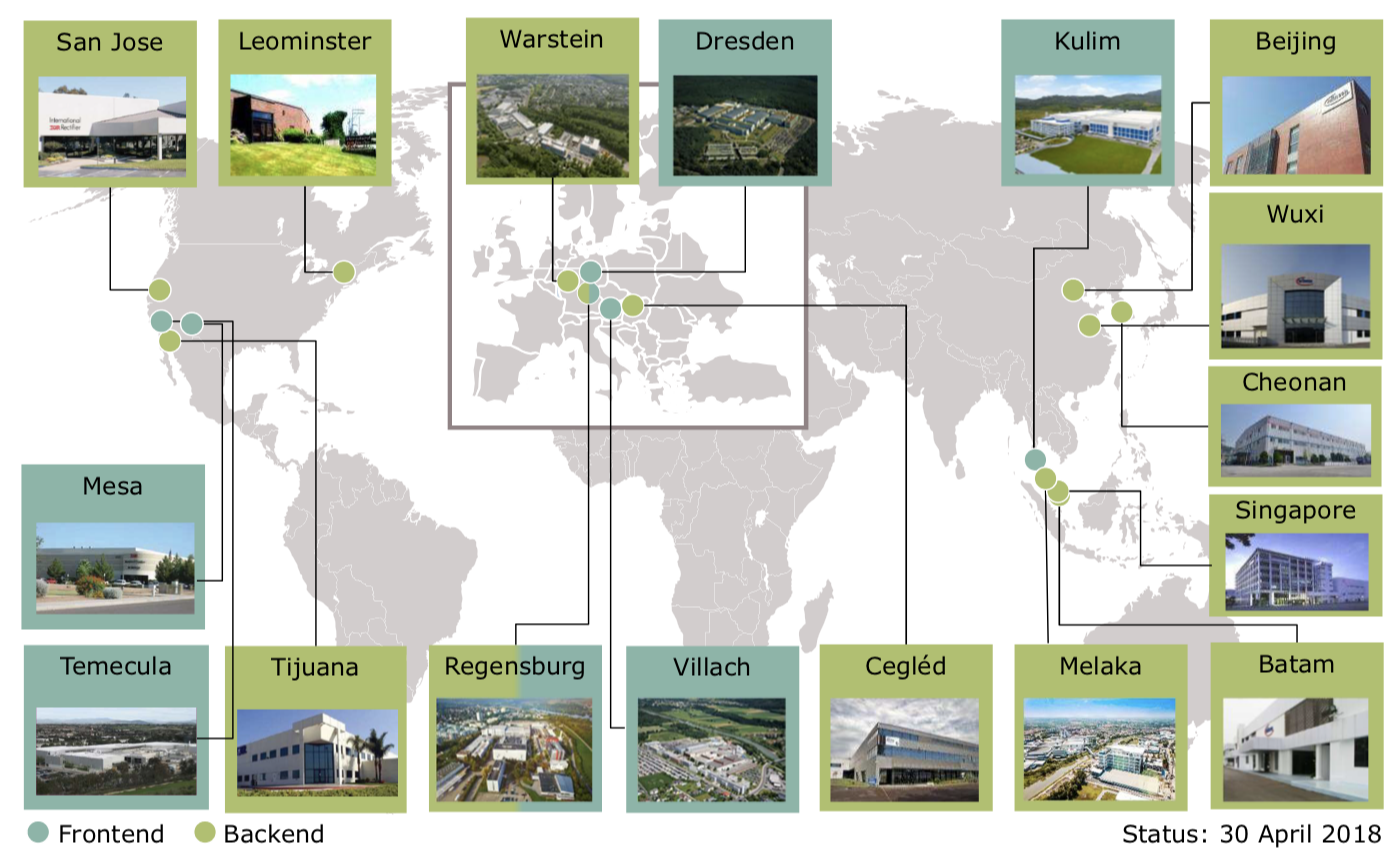
\includegraphics[width=\textwidth]{./settings/infineon}
	\caption[Produktionsstandorte im Infineon Produktionsnetzwerk]{Produktionsstandorte im Infineon Produktionsnetzwerk\footnote{Eigene Abbildung.}}\label{fig:ifx}
\end{figure}

Jeder Wafer hat dabei ein spezielles Rezept (Operationsreihenfolge) und wird in dieser Reihenfolge auf unterschiedlichen Maschinen bearbeitet. Selbst die Annahme, dass Rüstzeiten aus der Betrachtung ausgeschlossen werden, trifft bei fast allen Prozessen aufgrund einem hohen Automatisierungsgrad zu.


\chapter{Mathematische Problemformulierung}

Bei der mathematischen Formulierung des Distributed Job Shops $DJ_m$ wird folgende Notation nach \cite{pinedo-scheduling} verwendet:

\begin{itemize}
	\item $n$ — Anzahl an der Jobs $j,k = \{0,1,2,\ldots, n\}$, wobei es sich bei job 0 um einen Dummy Job zur Identifizierung des ersten auf einer Maschine zu prozessierenden Jobs handelt
	\item $m$ — Anzahl der Maschinen $i, l = \{1, 2, \ldots, m\}$
	\item $f$ — Anzahl der Produktionsstätten $r = \{1, 2, \ldots, f\}$
	\item $p_{j,i}$ — Porzessierungszeit von Job $j$ auf Maschine $i$
\end{itemize}

Nach Pinedo sollte das Scheduling Problem durch ein Triplet aus Maschinenumgebung, Prozesscharakteristiken und Zielfunktion beschrieben werden. Im Falle des Distributed Job Shops kann das Problem wie folgt beschrieben werden:

\begin{equation}
J_{f,m} | | C_{max}
\end{equation} \\
Im Gegensatz zum klassischen Job Shop Problem, was durch $J_{m} | | C_{max}$ beschrieben wird, muss im Distributed Job Shop die Produktionsstätte ebenfalls $f$ mit in Betracht gezogen werden.

\chapter{Verfahrenslösung}
\section{Regel-basierte Heuristiken}

Bei den Regel-basierten Heuristiken wird, wie im ersten Kapitel erklärt, in zwei Schritten vorgegangen. 

\subsection{Aufteilung von Jobs auf Produktionsstätten}
Bei der Aufteilung der Jobs auf die Produktionsstätte werden folgende Aspekte mit in Betracht gezogen:

\begin{itemize}
	\item Einbeziehung der Prozesszeiten je Auftrag $j$ auf den verschiedenen Maschinen als Kennzahl für Arbeitspensum
	\item Möglichst gleichmäßige Aufteilung der Prozesszeiten auf die jeweiligen Maschinen der Produktionsstätten (Ungleichverteilung kann zu schlechter Kapazitätsauslastung führen)
	\item Jobs mit gleichen Routen sollten auf verschiedene Produktionsstätten verteilt werden, da sie die Fertigungsdauer erhöhen können durch potenziell erhöhte Standzeiten
\end{itemize}

Diese Punkte wurden in der entwickelten Formel für die Kalkulation des Arbeitspensums berücksichtigt\footcite[S. 7756]{djs-modeling}:

\begin{equation}
\text{Arbeitspensum}(j,i)=\left(\sum_{k \in R_{j,i}} p_{j,k} \right) + p_{j,i} \text{  } \forall_{i j}
\end{equation}\\
wobei $R_{j,i}$ dem Satz aller der Maschine $i$ vorgeschalteten Maschinen aus Job $j$ entspricht. Bei der Verteilung von Jobs auf Fabriken soll das maximale Arbeitspensum je Fabrik und Maschine minimiert werden.

\begin{figure}[h]
	\centering
	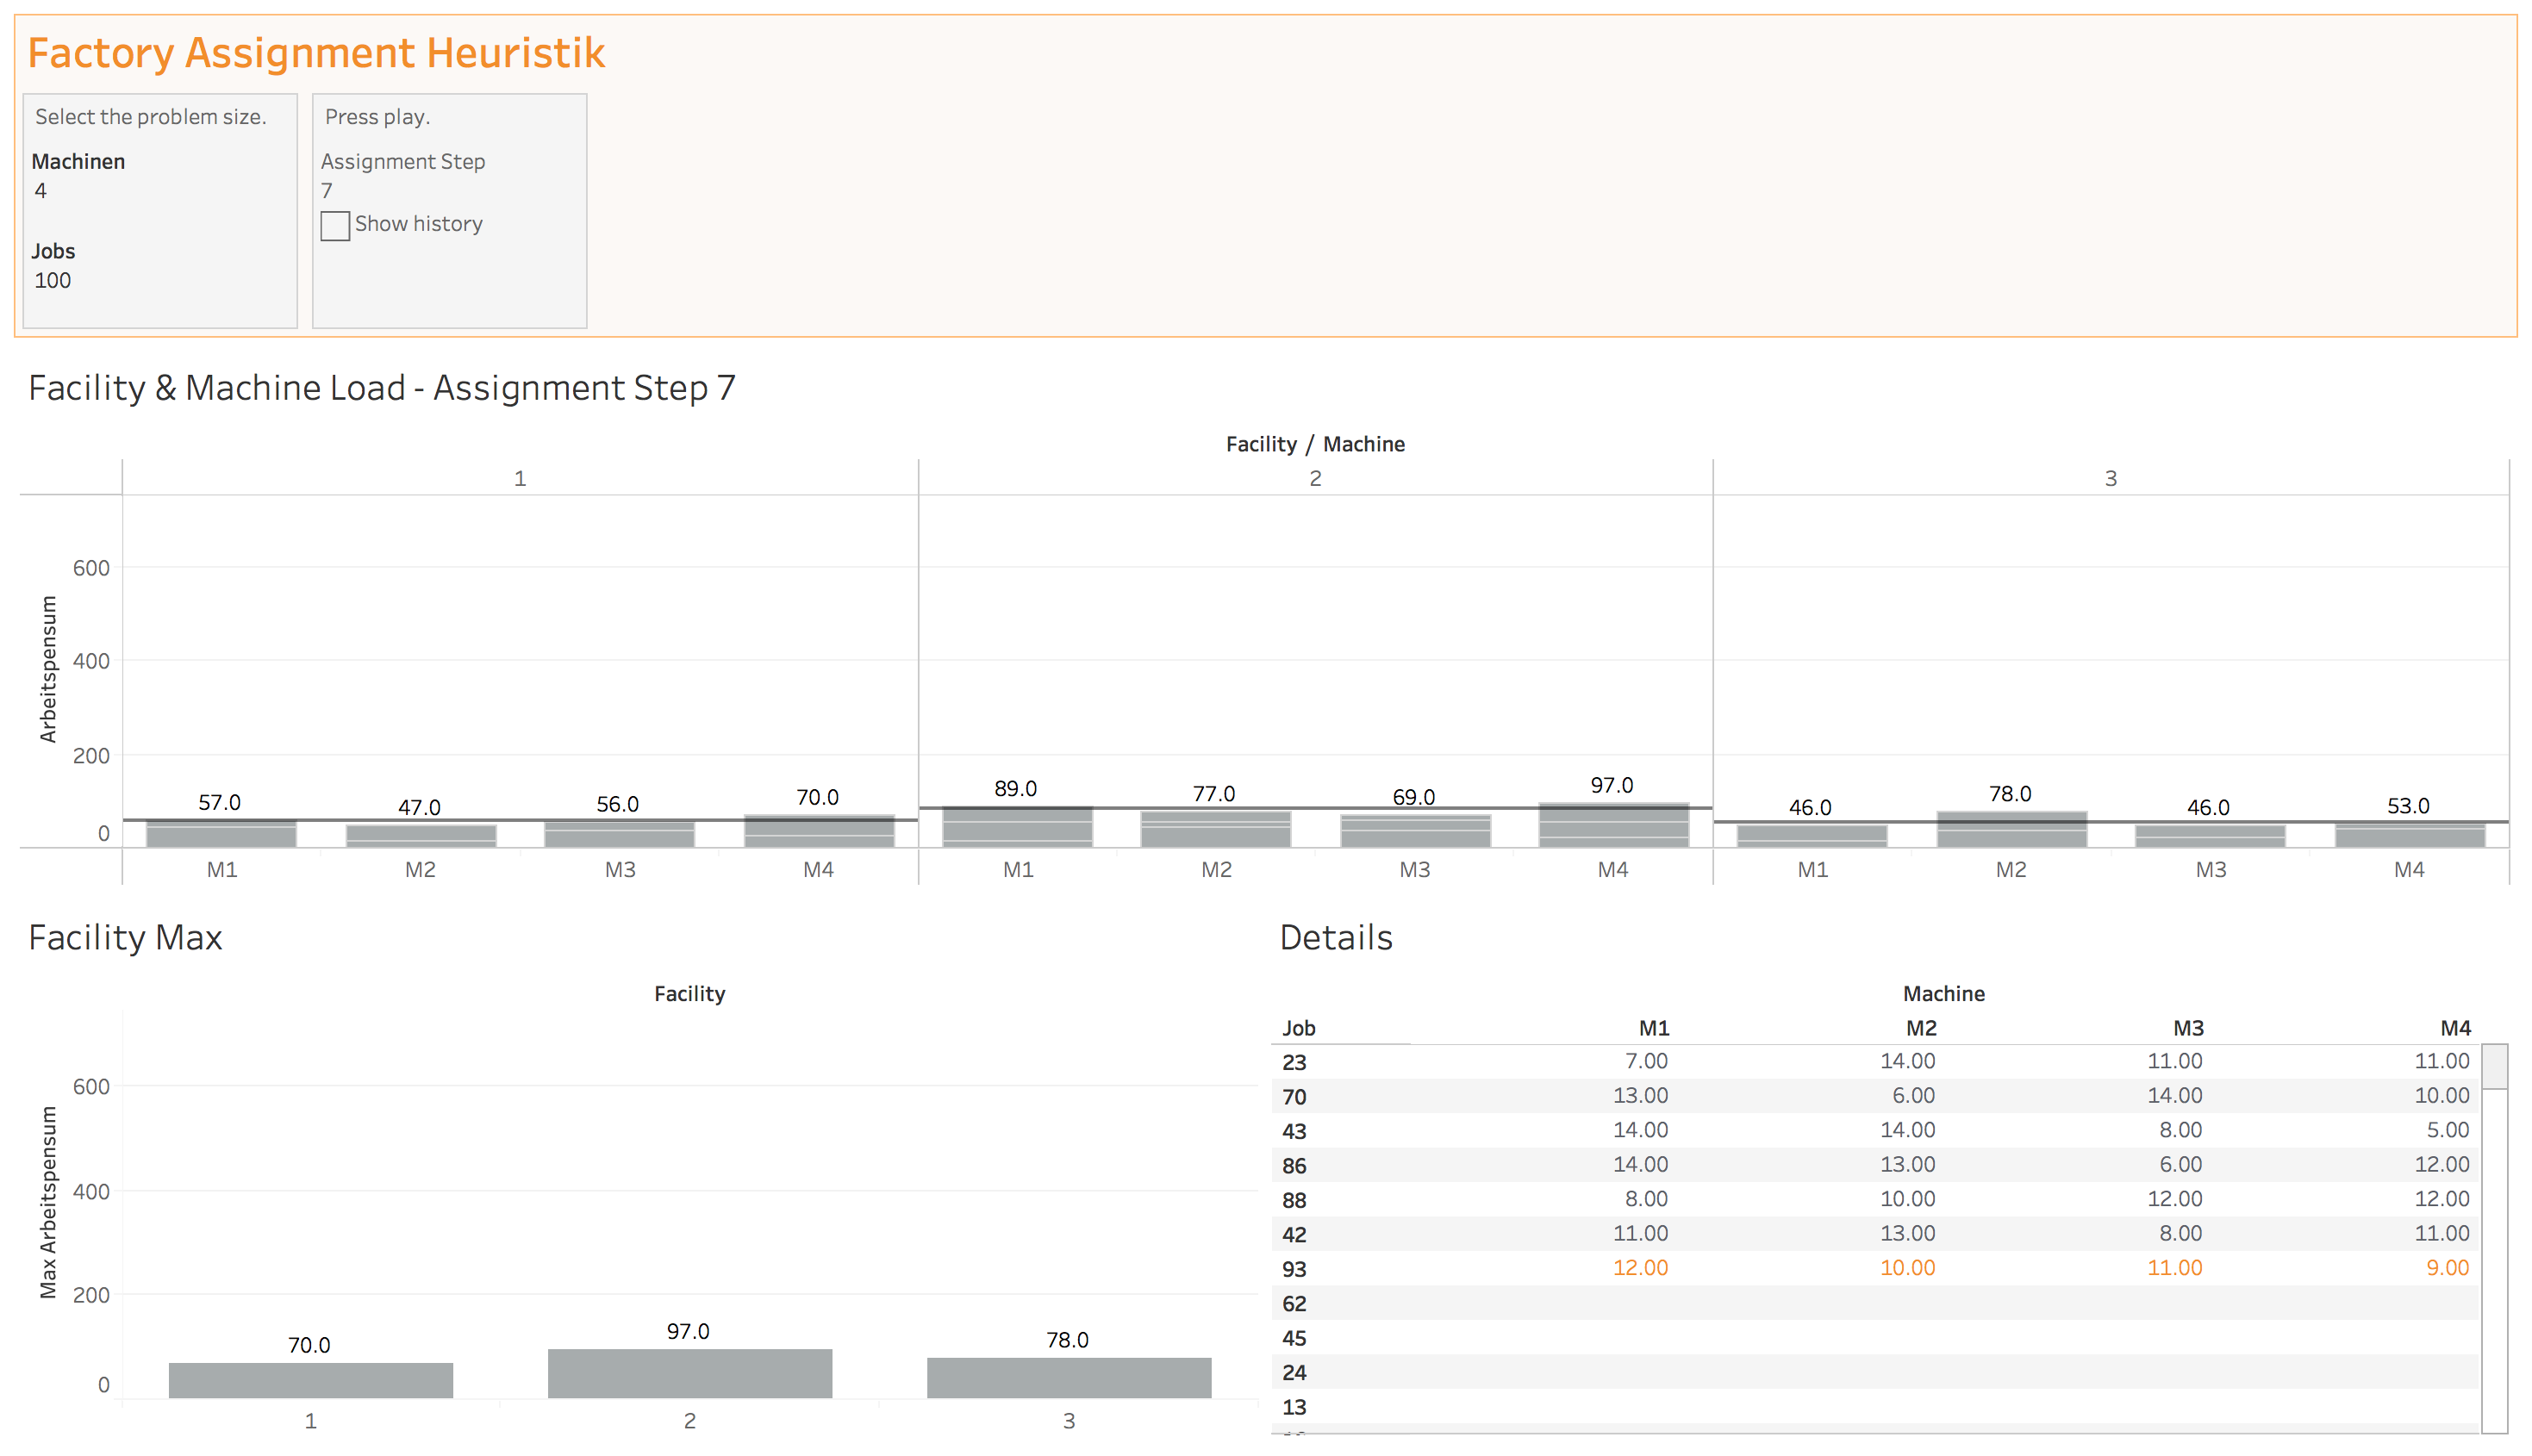
\includegraphics[width=\textwidth]{./settings/assignment}
	\caption[Zuordnung von Aufträgen zu Produktionsstandorten]{Graphische Aufbereitung der Zuordnung von Aufträgen zu Produktionsstandorten\footnote{Eigene Abbildung.}}\label{fig:assignment}
\end{figure}

\subsection{Einplanung der Aufträge auf Maschinen}
Mithilfe der bekannten Heuristiken \cgls{spt} und \cgls{lpt} (LPT) werden die den Produktionsstätten zugeordneten Jobs auf den einzelnen Maschinen eingeplant.

\subsection{Anwendungsbeispiel}
Im folgenden Problem sollen $j=4$ Jobs auf $f=2$ Produktionsstätten verteilt werden mit jeweils $m=3$ Maschinen. In Tabelle \ref{tab:problem} sind die Prozesszeiten der Jobs auf den Maschinen und deren Route angegeben. 

\begin{table}[H]
	\centering
	\begin{tabular}{ccccc}
		\toprule
		Job & M1 & M2 & M3 & Route \\
		\midrule
		1   & 3  & 7  & 4  & \{3, 2, 1\} \\
		2   & 6  & 5  & 3  & \{2, 1, 3\} \\
		3   & 12 & 1  & 6  & \{1, 3, 2\} \\
		4   & 2  & 9  & 5  & \{3, 2, 1\} \\
		\bottomrule
	\end{tabular}
	\caption{Jobs und Operationsfolge für das Anwendungsbeispiel}
	\label{tab:problem}
\end{table}

\subsubsection{Aufteilung von Jobs auf Produktionsstätten}
Mithilfe der Formel für Arbeitspensum kann dieses leicht errechnet werden. In der Tabelle \ref{tab:pensum} wird zusätzlich die Summe des Arbeitspensums für jeden Job berechnet und ein Rank nach absteigender Summe des Arbeitspensums vergeben.

\begin{table}[H]
	\centering
	\begin{tabular}{cccccc}
		\toprule
		Job & M1 & M2 & M3 & Summe & Rank \\
		\midrule
		1   & 11 + 3 = 14 & 4 + 7 = 11 & 0 + 4 = 4 & 29 & 4 \\
		2   & 11 & 5 & 14 & 30 & 3  \\
		3   & 12 & 19 & 18 & 49 & 1  \\
		4   & 16 & 14 & 5 & 35 & 2  \\
		\bottomrule
	\end{tabular}
	\caption{Ermitteltes Arbeitspensum und Rank}
	\label{tab:pensum}
\end{table}

Nach Ermittlung des Arbeitspensums und Ranks kann jetzt mit der Aufteilung der Jobs auf die einzelnen Produktionsstätten begonnen werden.\\

\noindent
\textbf{Iteration 1}\\
\noindent
Verteilung der ersten $f$ Jobs nach dem ermittelten Rank auf die Produktionsstätten und Bestimmung des maximalen Workloads auf der Produktionsstätte.

\begin{itemize}
	\item Job $j=3$ wird in Produktionsstätte $f=1$ gefertigt — maximaler Workload beträgt $19$.
	\item Job $j=4$ wird in Produktionsstätte $f=2$ gefertigt — maximaler Workload beträgt $16$.
\end{itemize}
\noindent
Die in dieser Iteration ermittelten Ergebnisse werden in Tabelle \ref{tab:aufteilung} eingetragen.\\

\noindent
\textbf{Iteration 2 … x}
\begin{enumerate}
	\item Ermittlung des nächsten nichtverteilten Jobs nach dem Rank
	\item Addition vom Arbeitspensum des Jobs zu dem jeweiligen bereits verteilten Arbeitspensum für die Produktionsstätten
	\item Ermittlung des Maximum des Arbeitspensums
	\item Verteilung des Jobs auf die Produktionsstätte mit dem minimalen Maximum
\end{enumerate}

\begin{table}[H]
	\centering
	\begin{tabular}{c p{2.5cm} c p{1.5cm} p{1.5cm} p{1.5cm} c c}
		\toprule
		Iteration & Produktions-stätte & Job & M1          & M2         & M3         & Max & Auswahl \\
		\midrule
		1            & 1                   & 3   & 12          & 19         & 18         & 19      & x       \\
					 & 2                   & 4   & 16          & 14         & 5          & 16      & x       \\
		\midrule
		2           & 1                   & 2   & 12 + 11 23   & 19 + 5 24  & 18 + 14 32 & 32      &         \\
					 & 2                   & 2   & 16 + 11 27  & 14 + 5 19  & 5 + 14 19  & 27      & x      \\
		\midrule
		3			& 1                   & 1   & 12 + 14 26  & 19 + 11 30 & 18 + 4 22  & 30      & x       \\
					 & 2                   & 1   & 27 + 14 41 & 19 + 11 30 & 19 + 4 23  & 41      &        \\
		\bottomrule
	\end{tabular}
	\caption{Arbeitstabelle zur Aufteilung von Jobs auf Produktionsstätten}
	\label{tab:aufteilung}
\end{table}

\noindent
Daraus ergibt sich, dass die Jobs wie folgt auf die Produktionsstätte verteilt werden:
\begin{enumerate}
	\item Jobs: {3, 1}
	\item Jobs: {4, 2}
\end{enumerate}

\subsubsection{Einplanung der Aufträge auf Maschinen mittels \cgls{spt} }
Zuerst Tabelle \ref{tab:spt1} erstellen und für jede Maschine nach der Prozesszeit aufsteigend sortieren.

\noindent
\textbf{Iteration 1 … x}
Jeweils die erste Zeile pro Maschine betrachten. Sind alle vorhergehenden Operationen abgeschlossen?

\begin{enumerate}
	\item Ja? Das Maximum aus ( Maximale Endzeit der Maschine, Maximale Endzeit des Jobs )ist die neue Startzeit. Die neue Endzeit ergibt sich aus der neuen Startzeit + Prozesszeit. Fortfahren mit nächster Maschine.
	\item Nein? Fortfahren mit nächster Zeile der Maschine.
\end{enumerate}

\noindent
Nach Durchführung des ersten Iterationsschrittes ergibt sich Tabelle \ref{tab:spt1}.

\begin{table}[H]
	\centering
	\begin{tabular}{c c c c c c}
		\toprule
		Machine & Job & Operation & Prozesszeit & Startzeit & Endzeit\\
		\midrule
		M1 & 1 & 3 & 3 & x &\\
		M1 & 3 & 1 & 12 & &\\
		M2 & 3 & 3 & 1 & x &\\
		M2 & 1 & 2 & 7 & &\\
		M3 & 1 & 1 & 4 & 0 & 4\\
		M3 & 3 & 2 & 6 & &\\
		\bottomrule
	\end{tabular}
	\caption{Ergebnis nach der ersten Iteration}
	\label{tab:spt1}
\end{table}

\noindent
Nach Durchführung aller Iterationsschritte ergibt sich Tabelle \ref{tab:spt2}.

\begin{table}[H]
	\centering
	\begin{tabular}{c c c c c c}
		\toprule
		Machine & Job & Operation & Prozesszeit & Startzeit & Endzeit \\
		\midrule
		M1 & 1 & 3 & 3 & 11 & 14\\
		M1 & 3 & 1 & 12 & 0 & 12\\
		M2 & 3 & 3 & 1 & 18 & 19\\
		M2 & 1 & 2 & 7 & 4 & 11\\
		M3 & 1 & 1 & 4 & 0 & 4\\
		M3 & 3 & 2 & 6 & 12 & 18\\
		\bottomrule
	\end{tabular}
	\caption{Einplanung der Jobs nach SPT}
	\label{tab:spt2}
\end{table}

\noindent
In der Präsentation wurde zu Illustrationszwecken unter anderem folgendes interaktives Beispiel verwendet:

\begin{figure}[H]
	\centering
	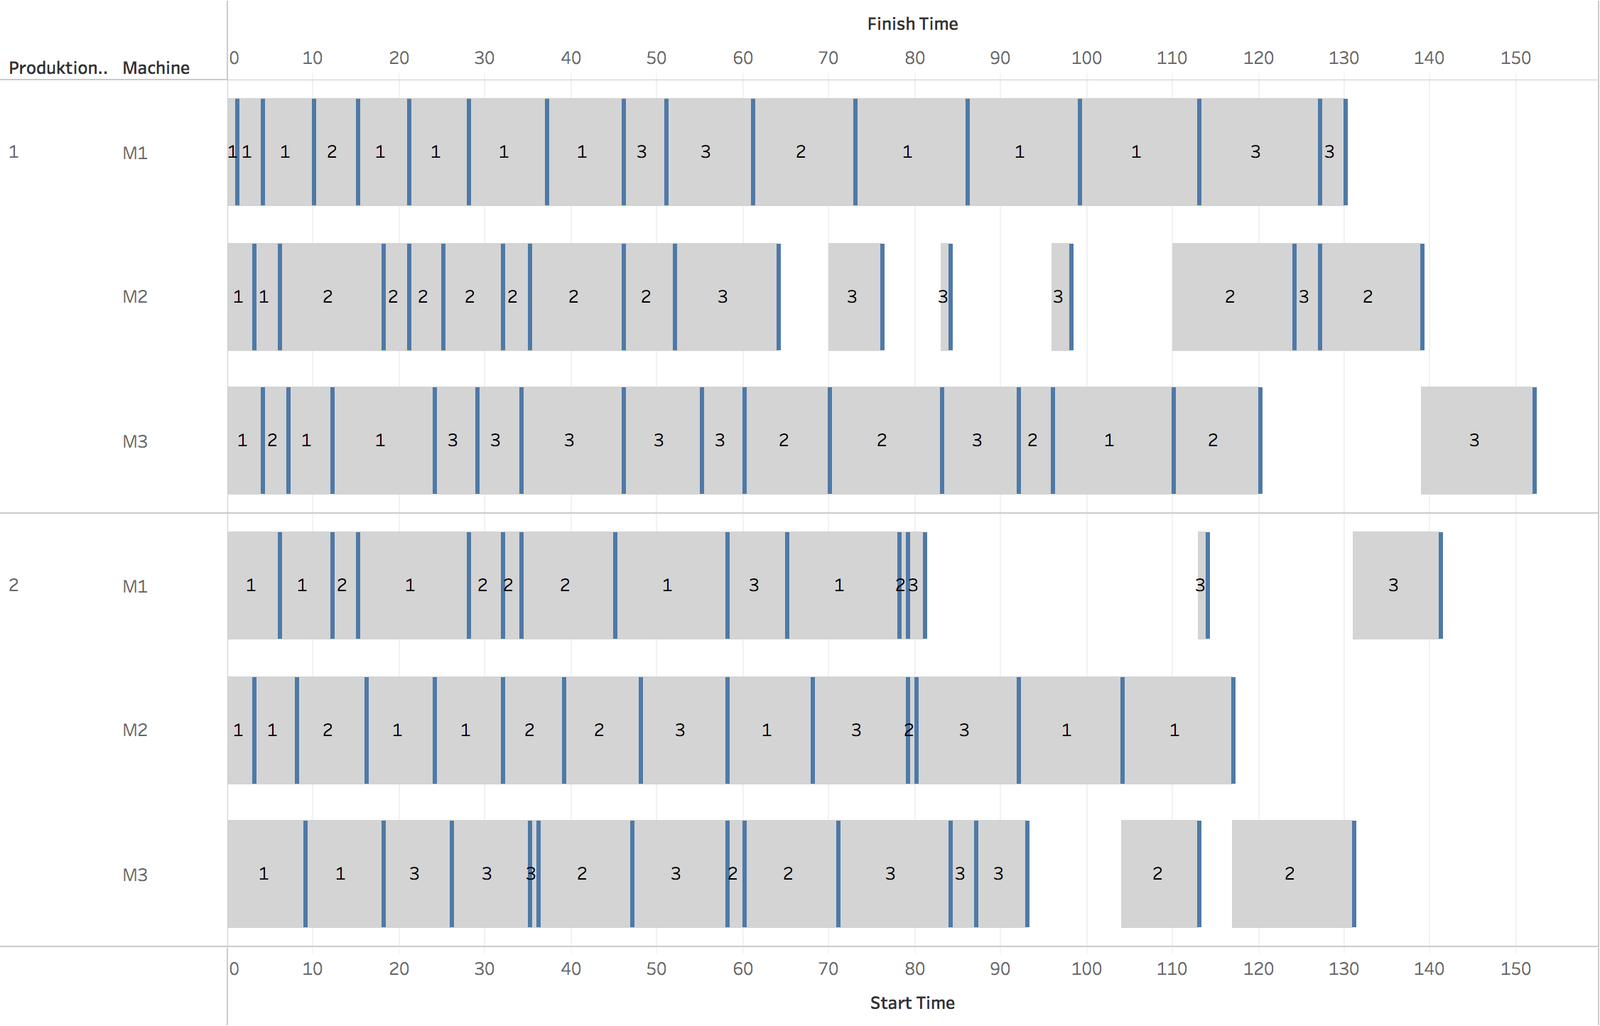
\includegraphics[width=\textwidth]{./settings/spt}
	\caption[Interaktives Beispiel - Einplanung nach der SPT Regel]{Darstellung der nach SPT eingeplanten Operationen im Gantt-Diagramm\footnote{Eigene Abbildung.}}\label{fig:spt}
\end{figure}

\noindent
\textbf{Longest Processing Time (LPT)}\\
\noindent
Die Schritte für LPT sind identisch zu den von SPT mit der Ausnahme, dass die Tabelle zu Beginn nicht aufsteigend, sondern absteigend sortiert wird. \\

\noindent
In der Präsentation wurde zu Illustrationszwecken unter anderem folgendes interaktives Beispiel verwendet:
\begin{figure}[H]
	\centering
	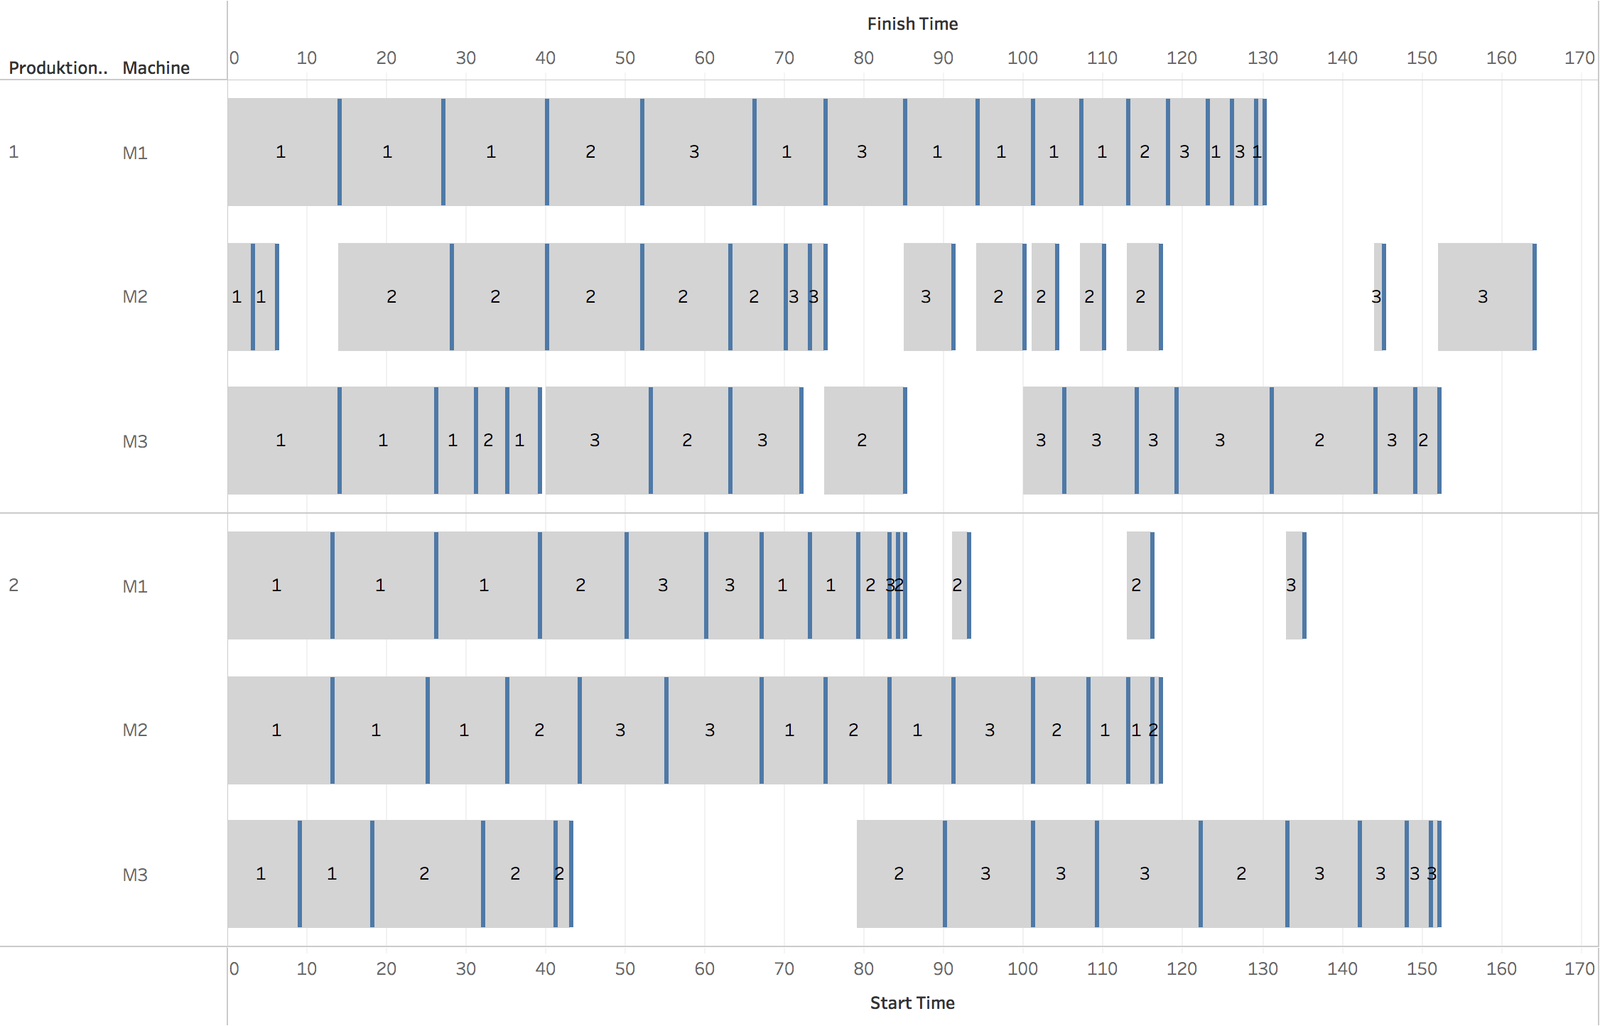
\includegraphics[width=\textwidth]{./settings/lpt}
	\caption[Interaktives Beispiel - Einplanung nach der LPT Regel]{Darstellung der nach LPT eingeplanten Operationen im Gant-Diagramm\footnote{Eigene Abbildung.}}\label{fig:spt}
\end{figure}


\section{Greedy Heuristiken}

Im “Modeling and heuristics for scheduling of distributed job shops” Paper von \cite{djs-modeling} werden weiterhin drei hoch-performante Greedy-Heuristiken eingeführt. Diese Heuristiken beruhen auf dem “insertion neighborhood concept”. D.h. es wird durch kontinuierliches Einsetzen eines Prozessschrittes an verschiedenen Stellen in der Prozesskette die Reihenfolge ermittelt, welche zur kürzesten Fertigungsdauer führt.

\subsection{Greedy-Heuristik 1}

\subsubsection{Allgemeines Vorgehen}
\noindent
\textit{Schritt 1.} Zuerst wird, wie im vorherigen Abschnitt eingeführt, die Zuteilung von Jobs auf die einzelnen Produktionsstätten mithilfe der Kenngröße des Arbeitspensums durchgeführt.\\

\noindent
\textit{Schritt 2.} Für jede Produktionsstätte wird eine zufällige Reihenfolge der Operationen (Operationsfolge) bestimmt, wobei eine spezielle Array-Datenstruktur verwendet wird. Anstatt sowohl Job, Machine und Operationsnummer zu verwenden, wird nur die Jobnummer verwendet welche $m$ Mal wiederholt wird. Durch die Position und die Anzahl der Vorkommnisse der Jobnummer vorher, kann wieder auf Maschine und Operationsnummer zurückgeschlossen werden. Produktionsstätte 1, aus dem vorher vorgestelltem Beispiel, wurde die Jobs $(1, 3)$ zugewiesen, wobei jeder der Jobs auf drei Maschinen bearbeitet wird. Somit ergibt sich, dass beide Jobnummer jeweils drei Mal vorkommen müssen. Die zufällige generierte Reihenfolge der Operationen könnte daher z.B. $[1,3,1,1,3,3]$ lauten. Das würde bedeuten, dass Job $1$ auf Maschine M3 bearbeitet wird, bevor mit der Bearbeitung von Job $3$ auf Maschine M1 begonnen wird.\\

\noindent
\textit{Schritt 3.} Für jede Produktionsstätte wird der Länge des Arrays entsprechend viele Iterationen durchgeführt. Der Laufindex $i$ wird für die Iterationszahl eingeführt und es wird die Variable $\text{best\_seq}$ verwendet, in der die beste ermittelte Operationsfolge gespeichert wird. Die Jobindizes werden nacheinander aus der ursprünglichen Operationsfolge genommen und in alle möglichen Positionen in der Operationsfolge getestet. Schließlich wird die beste Position ausgewählt. Die Prozedur wird für den nächsten Job wiederholt.

\subsubsection{Anwendungsbeispiel}
\noindent
Zufällige Operationsfolge: $[1,3,1,1,3,3]$\\

\noindent
\textbf{Iteration 1:}\\
\noindent
Es wird der Job an erster Stelle der Operationsfolge ermittelt — Job 1. Es gibt keine weiteren Jobindizes in $\text{best\_seq}$, weshalb $[1]$ als neue $\text{best\_seq}$ gespeichert wird.\\


\noindent
\textbf{Iteration 2:}
\begin{enumerate}
	\item Ermittle den Jobindex an der zweiten Stelle der originalen Operationsfolge. In unserem Fall wäre dies Job $3$.
	\item Da $\text{best\_seq}= 1$ entspricht ergeben sich folgende Permutationen: $\{ [1,3], [3,1] \}$. Nehmen wir an, dass Sequenz $[1,3]$ die bessere ist — $\text{best\_seq}$ entspricht nun $[1,3]$.
\end{enumerate}

\noindent
\textbf{Iteration 3:}

\begin{enumerate}
	\item Ermittle den Jobindex an der dritten Stelle der originalen Operationsfolge. In unserem Fall ist dies Job $1$.
	\item Da wir bereits im vorherigen Schritt festgestellt haben, dass $[1,3]$ die beste Sequenz war, müssen nicht mehr alle Permutationen getestet werden. Stattdessen müssen nur noch Permutationen getestet werden, die durch einsetzen des Jobindexes an jeder Position der $\text{best\_seq}$ generiert werden. Es ergeben sich daher folgende relevante Permutationen: $\{ [1,1,3], [1,1,3], [1,3,1] \}$.
	\item Es werden wieder die Permutationen getestet und die Beste wird in $\text{best\_seq}$ gespeichert.
\end{enumerate}

\noindent
\textbf{Iteration 4 … x:}\\
\noindent
Es werden die Schritte aus Iteration 3 wiederholt. \\

\noindent
\textbf{Testen von Operationsfolgen}\\
\noindent
Operationsfolgen werden wie folgt eingeplant und getestet:

\begin{enumerate}
	\item Über die gegebene Operationsfolge wird durch die Position des Jobindexes und Anzahl der vorher vorkommenden identischen Jobindizes die Maschine ermittelt. Basierend auf Operationsfolge $[1,1,3]$ kann auf folgende Informationen geschlossen werden:
	
	\begin{table}[H]
		\centering
		\begin{tabular}{c c c c }
			\toprule
			Job & Machine & Operation & Prozesszeit \\
			\midrule
			 1   & M3      & 1         & 4           \\
			 1   & M2      & 2         & 7           \\
			3   & M1      & 1         & 12          \\
			\bottomrule
		\end{tabular}
		\caption{Operationen in der zu betrachtenden Operationsfolge}
		\label{tab:greedyh11}
	\end{table}

	\item In der durch die Operationsfolge bestimmten Reihenfolge werden die Jobs auf den Maschinen eingeplant. Der Startzeitpunkt auf der jeweiligen Maschine entspricht dem Maximum des letzten Endzeitpunktes der Maschine und des Jobs.
	
	\begin{table}[H]
		\centering
		\begin{tabular}{c c c c c c }
			\toprule
			Job & Machine & Operation & Prozesszeit & Startzeit & Endzeit \\
			\midrule
			1   & M3      & 1         & 4           & 0         & 4       \\
			1   & M2      & 2         & 7           & 4         & 11      \\
			3   & M1      & 1         & 12          & 0         & 12      \\
			\bottomrule
		\end{tabular}
		\caption{Operationen in der zu betrachtenden Operationsfolge}
		\label{tab:greedyh12}
	\end{table}
	\item Der Maximale Endzeitpunkt entspricht der Fertigungsdauer. Es wird die Sequenz mit der geringsten Fertigungsdauer in jeder Iteration gewählt.
\end{enumerate}
\noindent
Im Folgenden findet sich ein Screenshot für das in der Präsentation verwendete interaktive Beispiel:
\begin{figure}[H]
	\centering
	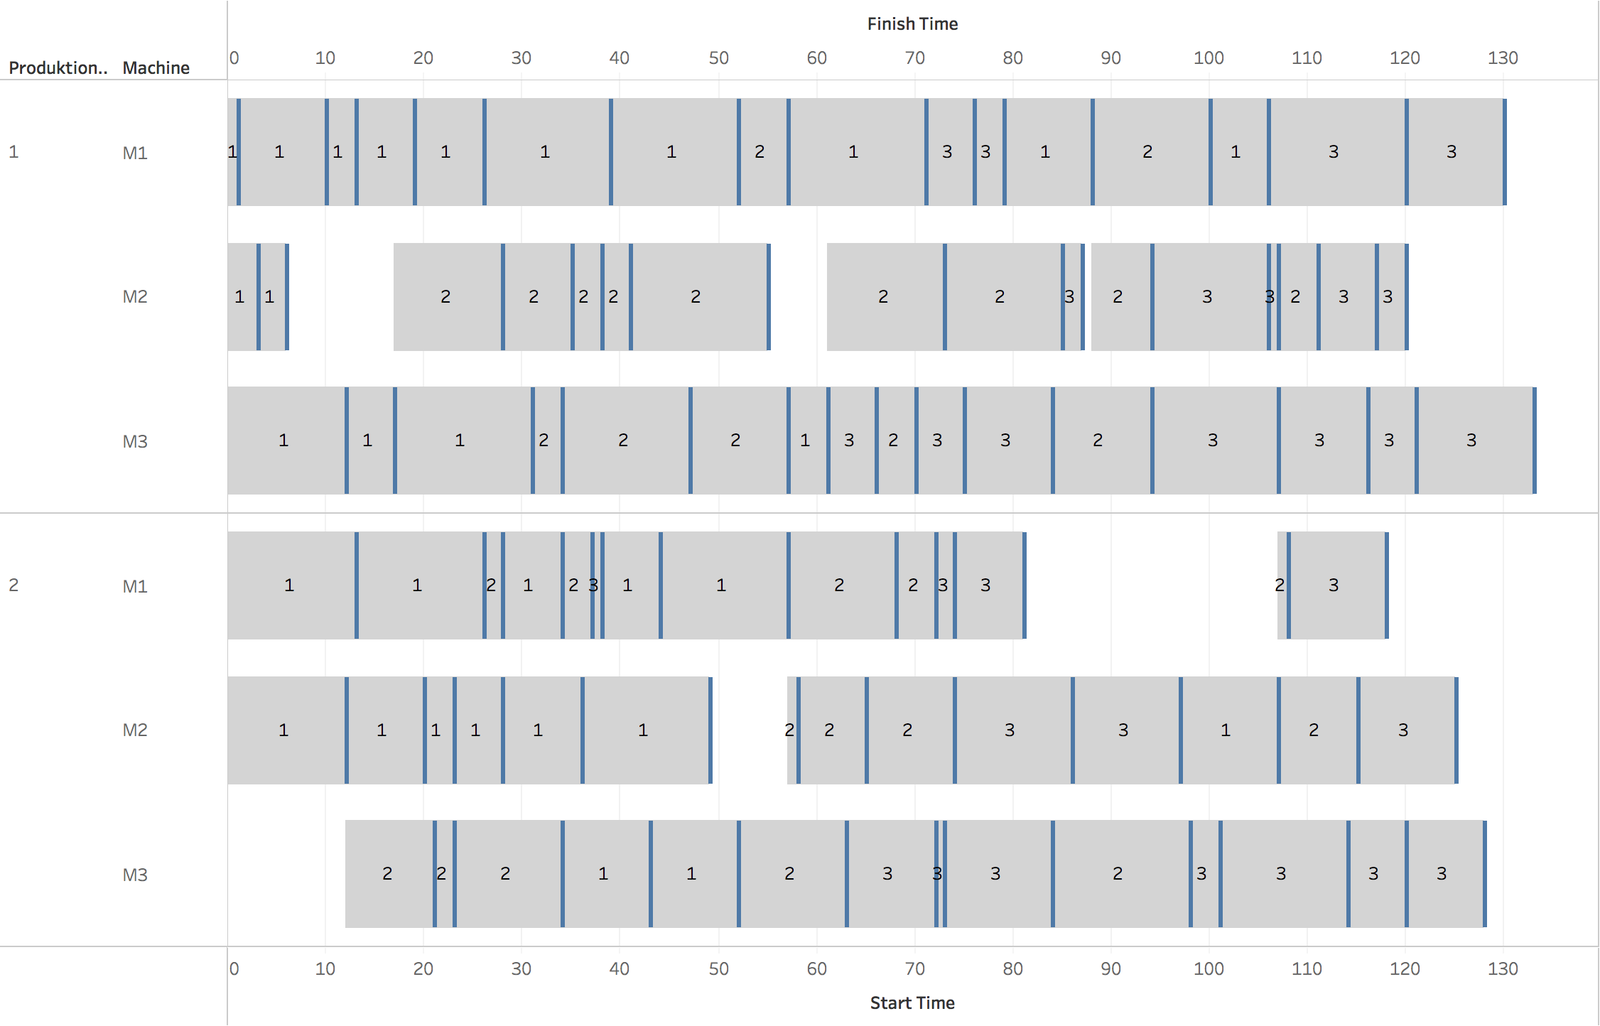
\includegraphics[width=\textwidth]{./settings/gh1}
	\caption[Interaktives Beispiel - Einplanung nach der ersten Greedy Heuristik]{Darstellung der nach der ersten Greedy Heuristik eingeplanten Operationen im Gant-Diagramm\footnote{Eigene Abbildung.}}\label{fig:gh1}
\end{figure}

\subsection{Greedy-Heuristik 2}

Die zweite Heuristik funktioniert ähnlich der ersten Heuristik. Der einzige Unterschied ist die Zuordnung der Jobs zu den Produktionsstätten. \\

\noindent
\textit{Schritt 1.} Zuerst wird die Liste der Jobs absteigend nach der Fertigungsdauer sortiert. Die ersten $f$ Jobs werden jeweils einer Produktionsstätte zugeordnet. \\

\noindent
\textit{Schritt 2.} Die restlichen Jobs werden weiter in der absteigenden Reihenfolge bearbeitet und jeweils der Produktionsstätte mit der niedrigsten gesamten Fertigungsdauer zugeordnet. Es wird nun der dritte Schritt aus der ersten Greedy-Hseuristik angewendet. \\

\noindent
Im Folgenden findet sich ein Screenshot für das in der Präsentation verwendete interaktive Beispiel:
\begin{figure}[H]
	\centering
	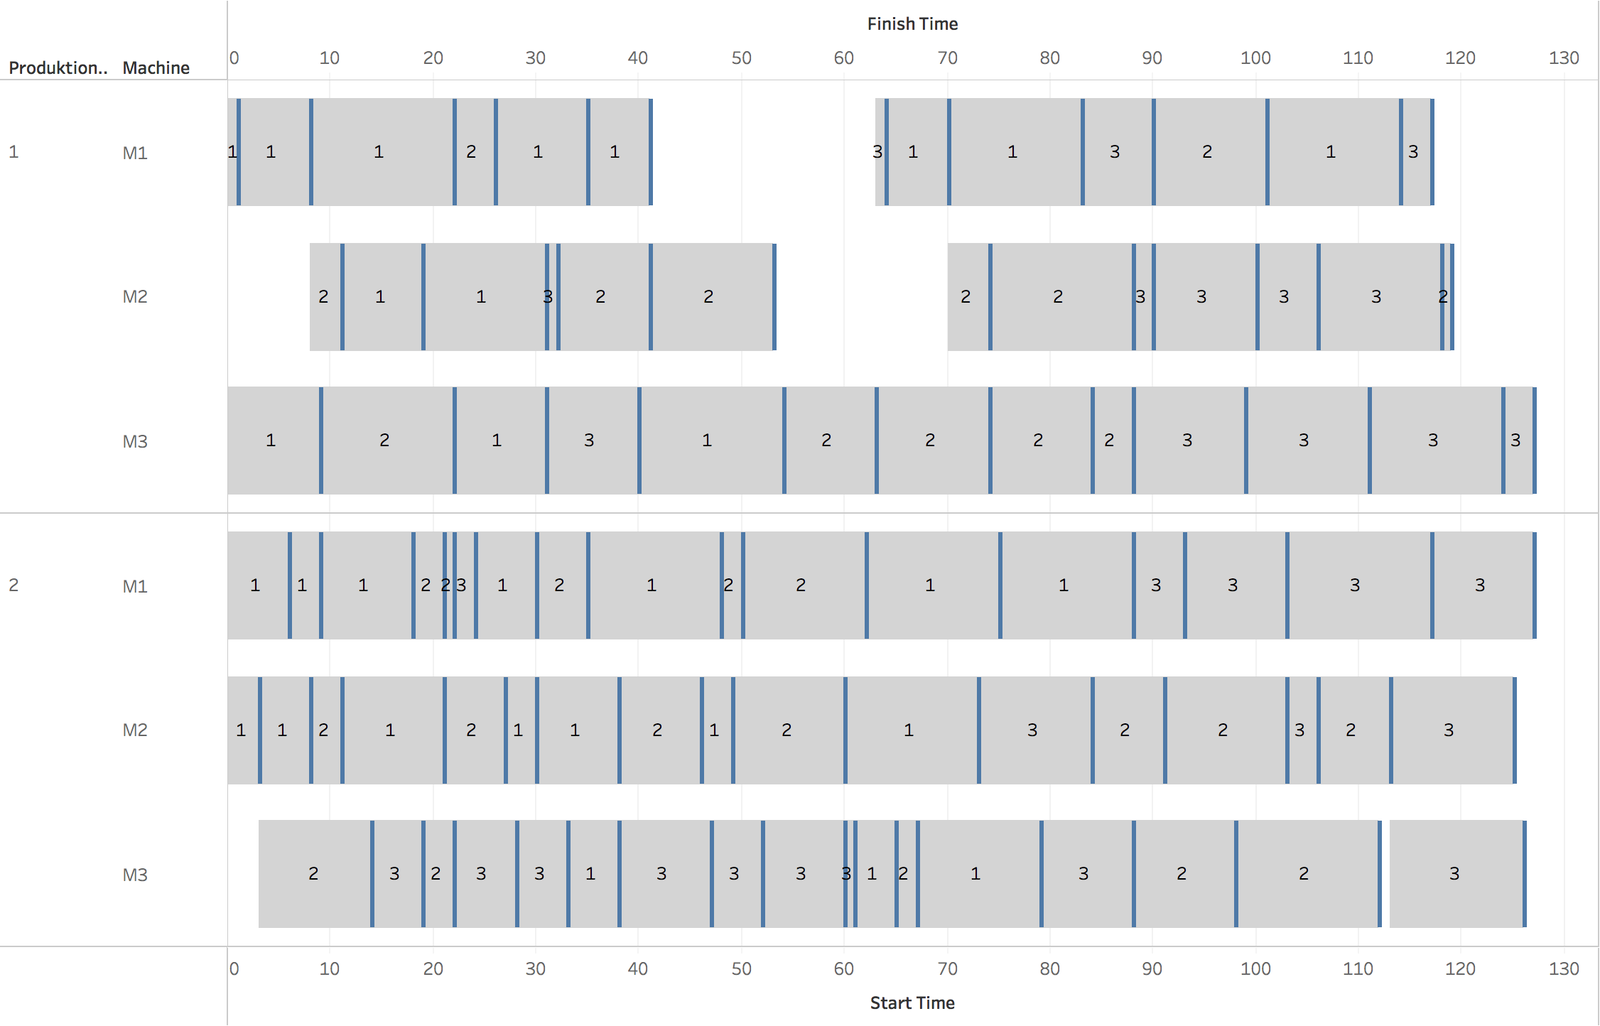
\includegraphics[width=\textwidth]{./settings/gh2}
	\caption[Interaktives Beispiel - Einplanung nach der zweiten Greedy Heuristik]{Darstellung der nach der zweiten Greedy Heuristik eingeplanten Operationen im Gant-Diagramm\footnote{Eigene Abbildung.}}\label{fig:gh2}
\end{figure}

\subsection{Greedy-Heuristik 3}
Die dritte Heuristik funktioniert ebenfalls ähnlich der ersten Heuristik. Der Unterschied ist, dass alle Permutationen inklusive die Zuordnung zu allen Produktionsstätten in jeder Iteration getestet wird.\\

\noindent
\textit{Schritt 1.}  Zuerst wird die Liste der Jobs erstellt. Dabei erfolgt keine Sortierung.\\

\noindent
\textit{Schritt 2.} Für jede Kombination aus Job und Fabrik wird der dritte Schritt aus der ersten Greedy Heuristik angewendet. Der Job wird der Fabrik zugeordnet, dessen Fertigungsdauer am Ende minimal ist. \\

\noindent
Im Folgenden findet sich ein Screenshot für das in der Präsentation verwendete interaktive Beispiel:
\begin{figure}[H]
	\centering
	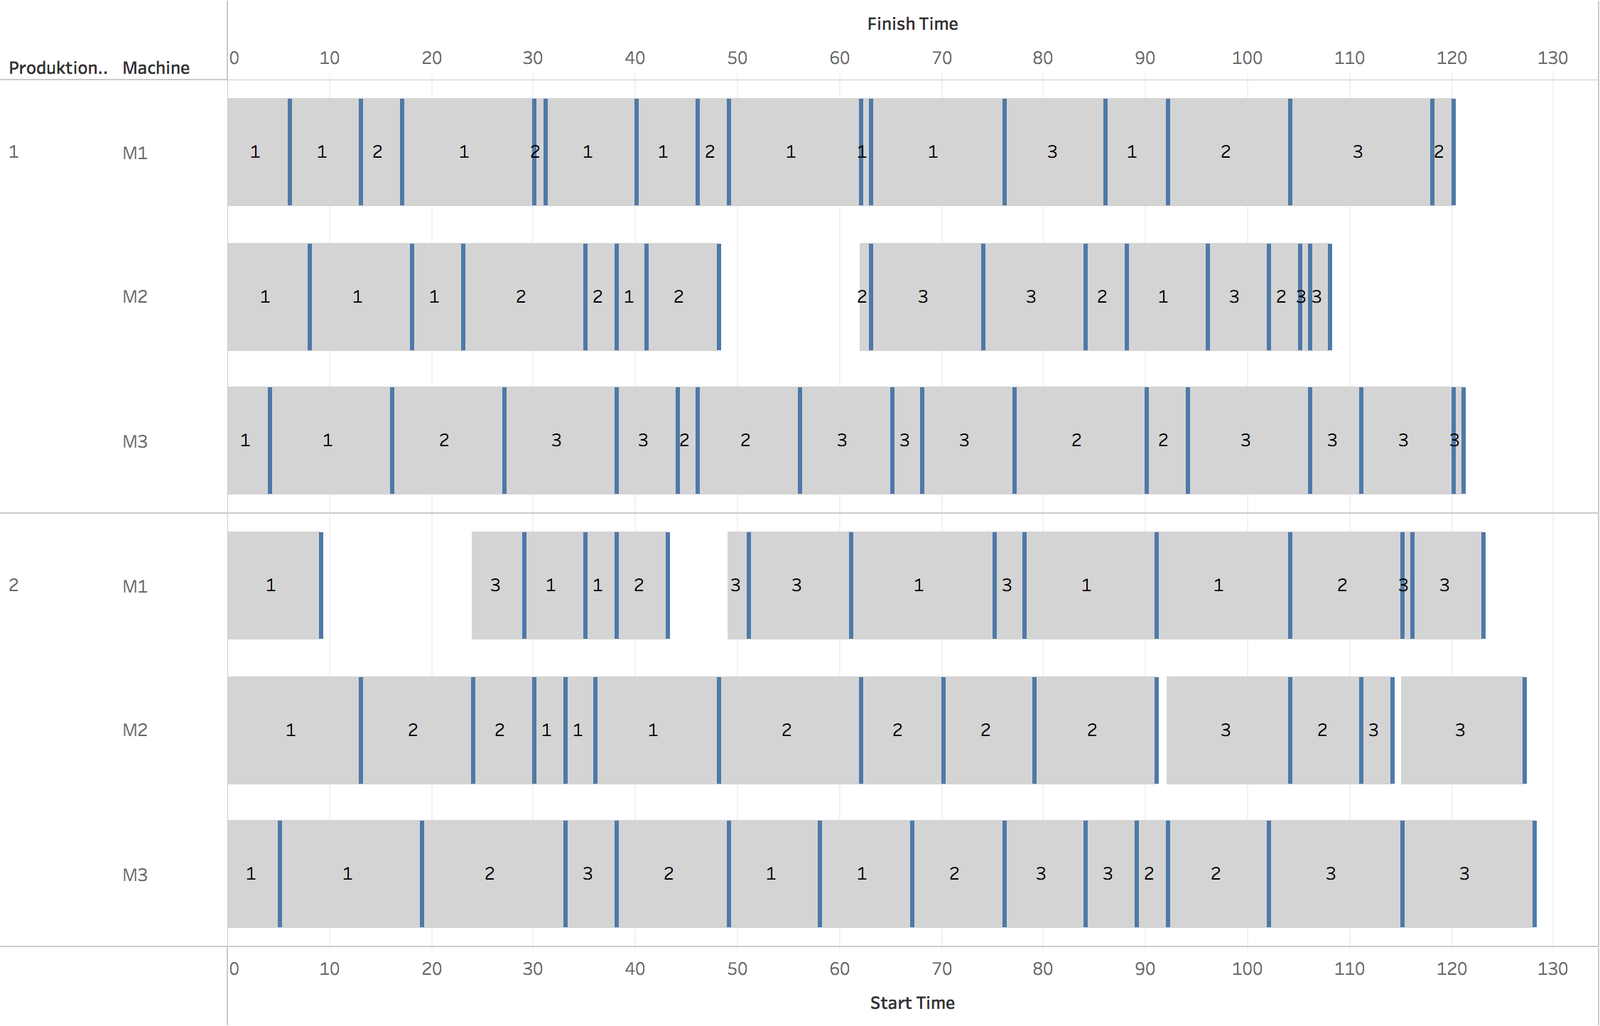
\includegraphics[width=\textwidth]{./settings/gh3}
	\caption[Interaktives Beispiel - Einplanung nach der dritten Greedy Heuristik]{Darstellung der nach der dritten Greedy Heuristik eingeplanten Operationen im Gant-Diagramm\footnote{Eigene Abbildung.}}\label{fig:gh3}
\end{figure}

%############################# Anhang #################################
\appendix

\chapter{Programmcodes}
Der Programmcode, welche im Rahmen dieser Arbeit entwickelt wurde, wurde auf \href{https://git.io/vhTVh}{GitHub} (https://git.io/vhTVh) veröffentlicht und kann unter der MIT License kostenfrei weiter- und wiederverwendet werden.


\clearpage

%####################### Literaturverzeichnis #########################
\addcontentsline{toc}{chapter}{\bibname}
\printbibliography

%####################### Selbständigkeitserklärung ####################
%\confirmation[place=Dresden] % Selbständigkeitserklärung

\end{document}